\chapter{Benders decomposition}

\section{Introduction}

Benders decomposition is a solution method for solving certain large-scale optimization problems. It is particularly suited for problems in which a set of variables are said to be \textit{complicating} in the sense that fixing them to a given value makes the problem easy. Briefly, the Benders decomposition approach seperates an original problem into several decision stages. A first-stage \textit{master} problem is solved using only a subset of variables, then, the values of the remaining variables are determined by a so-called \textit{subproblem} depending on the first-stage variables. If the master problem's optimal solution yields an infeasible subproblem, a \textit{feasibility cut} is added to the master problem, which is then re-solved. Due to the structure of the reformulation, the Benders algorithm starts with a \textit{restricted master problem} where only a subset of constraints are considered while the others are iteratively added. 

This technique was first introduced in \cite{Benders1962} and has since been generalized to non-linear mixed integer problems. 

\section{Formal derivation}

Consider the following problem :
\begin{align}
    \textrm{minimize } & c^Tx + f(y) \\
    \textrm{s.t. } & Ax + g(y) = b \\
    & y\in Y, x\ge 0
\end{align} where variable $y$ is a \textit{complicating constraint}. Note that it may be complicating due to the form of $f$ or $g$ but also by our ability to enforce the constraint $y\in Y$. We assume that fixing $y$ to a given value $\hat y$ turns our problem into an easy-to-solve problem. 

We can notice that our problem is equivalent to the following one : \[
    \min\left\{ f(y) + \min\left\{ c^Tx : Ax = b - g(y) \right\} : y \in Y \right\}
\] Let us denote by $q(y)$ the value of the minimization problem over $x$ : $q(y) = \min\{ c^Tx : Ax = b - g(y) \}$. By duality, the following holds \[
    q(y) = \max\{ (b-g(y))^T\pi : A^T\pi \le c \}
\] Note that the feasibility space of the dual does not depend on the values of $y$ and let us apply the decomposition theorem for polyhedra \ref{th:decomposition_polyhedra} on it :
\begin{align*}
    &\{ A^T\pi \le c \} = \left\{ \sum_i u^i\alpha_i + \sum_j v^j\beta_j \right\} \\
    &\sum_i \alpha_i = 1 \quad\textrm{and}\quad \alpha, \beta \ge 0
\end{align*} where $\{u^i\}_i$ denotes the extreme points of $\{x|Ax\le c\}$ and $\{v^j\}_j$ denotes the extreme rays of the polyhedral cone $\{x|Ax\le 0\}$. Intuitively, the convex combination of the extreme points of $\{x|Ax\le c\}$ defines the optimal solutions (since we know that there exists at least one optimal solution corresponding to an extreme point of the considered polyhedron) while the conical combination of extreme rays of $\{x|Ax\le 0\}$ defines the feasibility region. The following theorem will allow us to reformulate our problem :
\begin{theorem}
    \label{th:upper_bounded_problem_theorem}
    Let ($\mathcal P$) be the following problem : \[ \max\{ c^Tx : Ax \le b, x\ge 0 \} \tag{$\mathcal P$} \] Then, ($\mathcal P$) is upper bounded if and only if 
    \[ c^Tv^j \le 0\quad \forall j=1,...,J \]
    where $\{v^j\}_{j=1,...,J}$ denotes the set of extreme rays of $\{x|Ax\le 0\}$. 
\end{theorem}
\begin{proof}
$\Rightarrow$ : By contradiction, let us suppose that $(\mathcal P)$ is upper bounded and that there exists $k$ such that $c^Tv^k > 0$. Let us consider a feasible solution to ($\mathcal P$) denoted by $u = z + t$ where $z$ is a convex combination of the extreme points of $\{x|Ax\le b\}$ and $t$ an element of the conical combinations of the extreme rays of $\{x|Ax\le 0\}$ (see theorem \ref{th:decomposition_polyhedra}). Let $\lambda\in\R_+$. Since $v^k$ is in the conical polyhedra $\{x|Ax\le 0\}$, it holds that $\lambda Av^k\le 0$. Moreover, we have $At\le 0$. Hence, $A(t+\lambda v^k)\le 0$. Now, since $v^k\ge 0$, we have $\lambda v^k\ge 0$ and since $t\ge 0$ it holds that $t+\lambda v^k\ge 0$. This shows that, for any $\lambda$, $z+\lambda v^k$ is a feasible solution for problem ($\mathcal P$). However, its associated objective value is given by $c^Tu + \lambda c^Tv^k\rightarrow +\infty$ when $\lambda\rightarrow+\infty$ since, by assumption, $c^Tv^k> 0$. This contradicts the fact that ($\mathcal P$) is upper bounded. \\
$\Leftarrow$ : Let us consider a solution $u = z + t$ then $c^Tu = c^Tz + \sum_j c^Tv^j\beta_j \le c^Tz$ since $c^Tv^j\le 0, \forall j=1,...,J$. Problem ($\mathcal P$) is therefore upper bounded by $\sum_i \alpha_i \max_i\{ c^Tu^i \}$. 
\end{proof}
Theorem \ref{th:upper_bounded_problem_theorem} can be intuitively understood by interpreting $c^Tv^j$ as $\langle c, v^j\rangle$ (scalar product). The necessary and sufficiant condition that $\langle c, v^j\rangle\le 0$ simply expresses that the the hyperplane defining the objective function must be \textit{oriented} (i.e., increasing) in the direction of the origin of the cone formed by the extreme rays of the polyhedron. It is depicted in figure \ref{fig:upper_bounded_problem}.

\begin{figure}[h!]
    \centering
    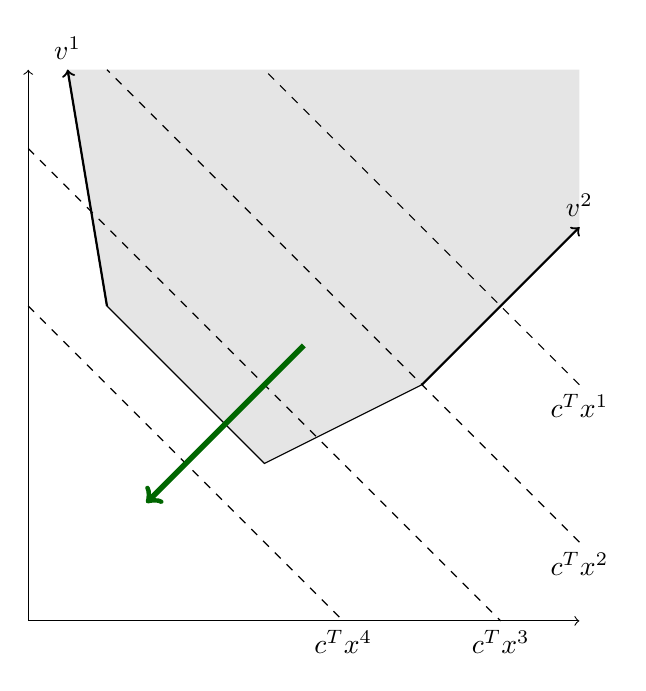
\begin{tikzpicture}
        \draw[<->] (7, 0) -| (0, 7);
        \fill[fill=gray!20] (.5,7) -- (1,4) -- (2,3) -- (3,2) -- (5,3) -- (7,5) -- (7,7) -- cycle;
        \draw (.5,7) -- (1,4) -- (2,3) -- (3,2) -- (5,3) -- (7,5);
        \draw[->, thick] (1,4) -- (.5,7) node[above] {$v^1$};
        \draw[->, thick] (5,3) -- (7,5) node[above] {$v^2$};

        \draw[dashed] (7,3) node[below] {$c^Tx^1$} -- (3,7);
        \draw[dashed] (7,1) node[below] {$c^Tx^2$} -- (1,7);
        \draw[dashed] (0,6) -- (6, 0) node[below] {$c^Tx^3$};
        \draw[dashed] (0,4) -- (4, 0) node[below] {$c^Tx^4$};
        \draw[line width=2pt, black!60!green,<-] (1.5,1.5) -- (3.5,3.5);
    \end{tikzpicture}
    \[ c^Tx^4 \ge c^Tx^3\ge c^Tx^2 \ge c^Tx^1 \]
    \caption{Illustration of theorem \ref{th:upper_bounded_problem_theorem}}
    \label{fig:upper_bounded_problem}
\end{figure}